\chapter{Introducción}\label{cap:1}
\lettrine{E}{n este capítulo, la misión principal} consiste en presentar, de forma clara y concisa, los fundamentos básicos que están detrás del presente Trabajo Fin de Máster. El contexto histórico aparece constantemente durante este proyecto, así como los protagonistas principales, sus descubrimientos y sus aportaciones más importantes en el marco del estudio realizado. De esta manera, se pretende que los futuros lectores puedan comprender las motivaciones y objetivos básicos perseguidos durante la ejecución del mismo.

En primer lugar, este trabajo está integrado dentro de una línea de investigación supervisada por el Dr. Eduardo Oliva Gonzalo ---ubicado en el Instituto de Fusión Nuclear \enquote{Guillermo Velarde} (IFN-GV)---, dedicada principalmente al análisis y modelización de la interacción láser-plasma para la generación y amplificación de rayos X blandos o radiación ultravioleta extrema. Los inicios de la investigación se remontan al comienzo de la tesis doctoral del Dr. Eduardo Oliva\autocite{olivaMejoraCodigoHidrodinamico2010}, para unos años después, en el año $2015$, comenzar a dirigir los primeros Trabajos Fin de Grado y Fin de Máster. Los trabajos realizados por Alba Guiomar Verdejo, Marina Ruiz Izu o Santiago López García guardan una relación estrecha con este trabajo, siendo la temática de este trabajo en cierta forma una continuación de estos, o aquellos antecesores de este.

Además, este estudio ha sido realizado en paralelo a las prácticas curriculares, supervisadas nuevamente por el Dr. Eduardo Oliva y revisadas por el Dr. Manuel Cotelo Ferreiro ---también ubicado en el IFN-GV---, destinadas principalmente a realizar tareas de modelización de armónicos de alto orden en plasmas mediante la escritura o modificación de programas, para después obtener y procesar las imágenes resultantes de las simulaciones. Los resultados y conclusiones presentados en los capítulos \S\ref{cap:4} y \S\ref{cap:5}, así como gran parte del trabajo de documentación y estudio realizado para la redacción, son fruto del tiempo empleado durante este periodo de prácticas.

En segundo lugar, los futuros lectores de este trabajo sentirán la necesidad de preguntarse por el título del mismo, su significado conjunto y el de los conceptos individuales que constituyen el estudio. La finalidad de este primer capítulo introductorio es satisfacer parcialmente estas preguntas a cerca de la naturaleza del TFM para después, en los capítulos \S\ref{cap:2} y \S\ref{cap:3}, terminar de presentar las ideas básicas que subyacen el proyecto y comenzar el análisis de los resultados en el capítulo \S\ref{cap:4}. Sin embargo, para orientar anticipadamente a los lectores, se presentan a continuación ---sin entrar en detalle--- las líneas básicas que aparecerán más detalladas posteriormente.

\begin{itemize}
  \item Láseres. A las escalas de energía e intensidad empleadas en la mayor parte de aplicaciones del mundo, es suficiente emplear un tratamiento clásico de la radiación láser. Dentro de este marco, es un sistema que produce ondas electromagnéticas con unas propiedades ópticas especiales, siendo el protagonista de una infinidad de aplicaciones científicas y tecnológicas como, por ejemplo, la fusión por confinamiento inercial o los interferómetros modernos. La sección \S\ref{sec:1.1} desarrolla estos sistemas en mayor profundidad.
  \item Rayos X blandos. También llamados radiación ultravioleta extrema, del inglés \emph{\acrfull{xuv}}, tienen longitudes de onda comprendidas entre los \qty{2}{nm} y \qty{20}{nm}. Los fenómenos ondulatorios que aparecen cuando una onda electromagnética interacciona con la materia ocurren gracias a que comparten longitudes de onda y tamaños característicos similares, motivando la utilización de radiación \acrshort{xuv} para observar escalas nanométricas, comunes por ejemplo entre familias de virus.
  \item Pulsos ultracortos y ultraintensos. Para visualizar correctamente escalas con un determinado tamaño, es necesario que la onda electromagnética deposite sobre la materia la cantidad de energía necesaria durante un intervalo de tiempo que permita obtener una resolución adecuada antes de inutilizar o destruir la muestra. La aparición a mediados de la década de los años ochenta de la técnica \acrshort{cpa}, del inglés \emph{\acrlong{cpa}}, desarrollada por Donna Strickland y Gérard Mourou\autocite{Strickland1985}, comenzó una nueva era de láseres capaces de proporcionar pulsos con energías de $\sim\unit{mJ}$ y $\sim\unit{fs}$ de duración, claves en un gran número de aplicaciones mencionadas a lo largo de este trabajo, incluido este último.
  \item Plasmas. El interés que despiertan está relacionado con la capacidad de ciertas especies de iones en plasmas densos de actuar como un medio amplificador de radiación \acrshort{xuv} en láseres basados en plasmas, especialmente cuando esta radiación son armónicos de alto orden. Las propiedades físicas y el comportamiento óptico de este estado de la materia aparece durante la sección \S\ref{sec:1.2}. 
  \item Armónicos de alto orden. Aparecen nombrados en la terminología inglesa como \emph{\acrfull{hoh}}. La generación de armónicos de alto orden, del inglés \emph{\acrfull{hhg}}, permite obtener armónicos ---ondas puras---, de radiación coherente con duraciones extremadamente cortas (pueden llegar a obtenerse pulsos de attosegundos) mediante la interacción de un láser muy intenso con un blanco generalmente gaseoso o sólido. Aunque individualmente son fuentes de radiación \acrshort{xuv} coherente con propiedades ópticas de gran importancia, explicadas en la sección \S\ref{sec:1.3}, combinar la inyección de armónicos de alto orden en plasmas densos permite obtener pulsos láser con características similares a los láseres de electrones libres (\acrshort{fel}), de mejores prestaciones que las demás fuentes por separado, pero reduciendo el tamaño y coste de las instalaciones. 
\end{itemize}

La síntesis de estos conceptos dan como resultado la posibilidad de utilizar armónicos de alto orden como una fuente de radiación \acrshort{xuv} coherente amplificada mediante su interacción con un plasma muy denso. Los capítulos \S\ref{cap:2} y \S\ref{cap:3} presentan esta conjunción de elementos en mayor profundidad, estando el plasma objeto de análisis durante este trabajo formado a partir de un gas de kriptón fuertemente ionizado, a través del cual viaja un armónico de alto orden para su amplificación y mejora de sus propiedades ópticas. 

Las discrepancias existentes entre múltiples experimentos llevados a cabo anteriormente y las simulaciones numéricas respecto a propiedades de la emisión \acrshort{xuv} obtenida son el centro de estudio del capítulo \S\ref{cap:4} y, esencialmente, el objetivo principal perseguido es reducir estas diferencias introduciendo modificaciones en los códigos disponibles y analizar los resultados observados.

\section{Láser}\label{sec:1.1}
En la actualidad, los láseres están presentes en una infinidad de aplicaciones científicas y tecnológicas. Muchas de estas aplicaciones son bien conocidas por la mayoría de la población general: procedimientos quirúrgicos en medicina y cirugía, mediciones de muy alta precisión, reconstrucción de imágenes tridimensionales ---conocida como holografía---, giroscopios de alta sensibilidad, escáneres de supermercados y reproductores CD, soldaduras y perforaciones de materiales, trazado de líneas rectas en superficies y topografía, litografía de materiales, telecomunicaciones y fibra óptica, y así sucesivamente.

En los primeros años de desarrollo, en la década de $1960$, existía un gran escepticismo sobre su aparición, siendo muchas las personas ---incluido el propio Maiman--- que calificaban esta tecnología como \enquote{una solución en busca de un problema}. Desde entonces han ido apareciendo muchos \enquote{problemas} como los mencionados, hasta convertir el láser en una parte fundamental de la ciencia y la tecnología de nuestro tiempo.  

La palabra láser o \emph{\acrfull{laser}} es un acrónimo de origen inglés empleado para describir el principio físico más fundamental que permite su funcionamiento, la amplificación de luz por emisión estimulada de radiación, de donde viene su nombre.

\subsection{Interacción radiación-materia}\label{sec:1.1.1}

\begin{equation}\label{eq:1.1}
  \nu_{0} = \frac{E_{2}-E_{1}}{h}
\end{equation}

\subsection{Propiedades ópticas}\label{sec:1.1.2}
La radiación emitida por un láser está caracterizada principalmente por una alta monocromaticidad, coherencia, direccionalidad e intensidad. A estas propiedades puede añadirse una quinta relacionada con la duración de la emisión\autocite{sveltoPrinciplesLasers2010}. Esta última hace referencia a la capacidad de generar pulsos de muy corta duración, propiedad que, aunque menos fundamental, tiene gran importancia en muchas aplicaciones. 

\paragraph{Monocromaticidad}\label{par:1.1.2.1}
De forma simplificada, esta propiedad se debe fundamentalmente a dos motivos: en primer lugar, solamente una onda electromagnética de frecuencia $\nu_0$ dada por \eqref{eq:1.1} puede ser amplificada y, en segundo lugar, como los esquemas de espejos utilizados forman una cavidad resonante, las oscilaciones pueden producirse únicamente a las frecuencias de resonancia de esta cavidad. Esta última circunstancia implica que el ancho de banda $\Delta\nu$ de la emisión láser es habitualmente mucho menor ---hasta diez órdenes de magnitud--- que el ancho de banda observado en la transición $2\rightarrow 1$ durante la emisión espontánea asociada.

Por ejemplo, las últimas propuestas de láseres de Fabry-Perot para la fabricación de circuitos integrados \autocite{tranExtendingSpectrumFully2022}, emplean frecuencias de \qty{300}{THz} ($\lambda = \qty{980}{nm}$) con anchos de banda $\Delta\nu = \qty{10}{kHz}$, resultando una anchura relativa para la frecuencia de emisión $\Delta\nu/\nu = 3,33\times 10^{-11}$. El espectro de la emisión láser tiene una alta pureza, como ilustra la Figura \ref{fig:ch1_amplif}, consiguiéndose reducir la dispersión a través de un medio de propagación dado y mejorando la focalización del haz, ya que el índice de refracción depende de la longitud de onda emitida.

\begin{figure}[ht!]
  \centering
  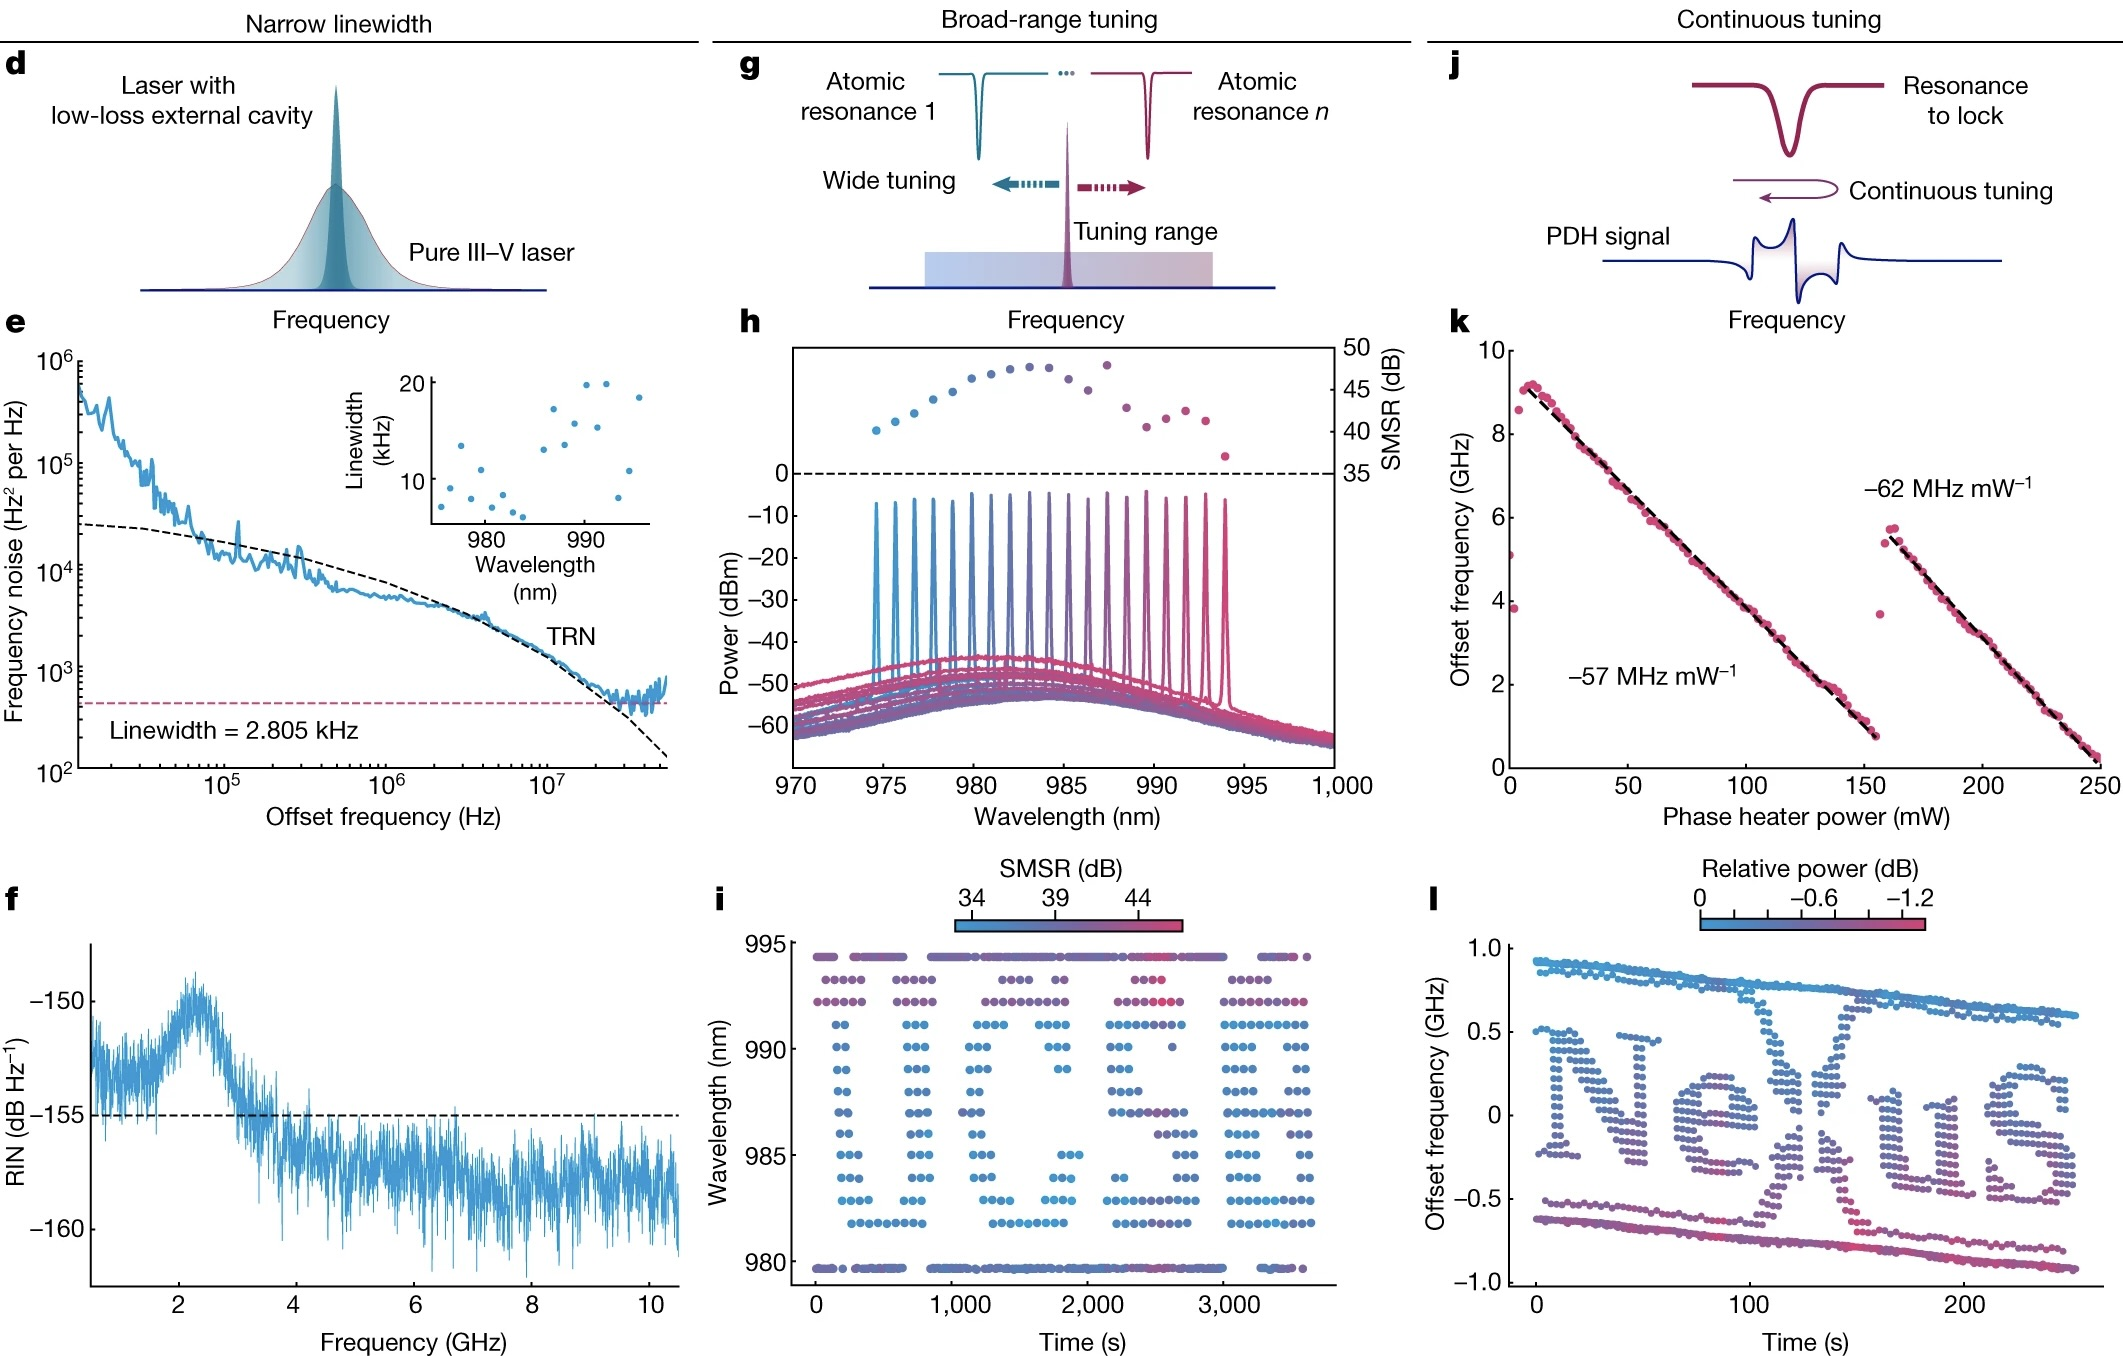
\includegraphics[width=\textwidth]{Figuras/ch1_amplif.png}
  \caption{Espectro de emisión del láser empleado en la propuesta\autocite{tranExtendingSpectrumFully2022}. \textbf{b}, Esquema del láser y sus elementos. \textbf{d}, Ancho de banda conseguido con la cavidad resonante. \textbf{e}, Ruido en la frecuencia del espectro de emisión. \textbf{g}, Frecuencias de resonancia. \textbf{h}, Longitudes de onda de operación.}
  \label{fig:ch1_amplif}
\end{figure}

En realidad, la longitud de onda de la transición láser admite ---por el principio de incertidumbre de Heisenberg--- frecuencias de excitación distintas a la ecuación \eqref{eq:1.1}, tal que $\nu_0\rightarrow\nu_0 + \delta\nu$. La magnitud de $\delta\nu$ es proporcional a la constante de Planck $h = \qty{6,626e-34}{J.s}$, siendo entonces extremadamente pequeña la variación introducida en el ancho de banda de la emisión láser debido a este fenómeno. 

Además, Schawlow y Townes demostraron que la anchura de banda mínima de un láser es la anchura de banda de la cavidad resonante dividida por dos veces el número de fotones $\langle n\rangle$ en el interior de la cavidad, límite conocido como \emph{\acrfull{sql}}. Sin embargo, existen grupos de investigación\autocite{liuProposalContinuousWave2021} que sugieren la posibilidad de utilizar circuitos superconductores para superar el \acrshort{sql} por un factor $\sim \xval{n}$ e incluso $\sim \xval{n}^{2}$, aproximándose al denominado \emph{límite de Heisenberg}.

\paragraph{Coherencia}\label{par:1.1.2.2}
A primer orden, el concepto de coherencia de una onda electromagnética introduce dos conceptos, llamados coherencia espacial y temporal\autocite{sveltoPrinciplesLasers2010}.

Para definir la coherencia espacial, basta con imaginar dos puntos $P_1$ y $P_2$ situados en el mismo frente de onda, en un instante inicial, de una onda electromagnética determinada, siendo $E_1(t)$ y $E_2(t)$ las amplitudes del campo eléctrico en dichos puntos. Por definición, el desfase entre ambos campos en ese instante es cero. Ahora bien, si en cualquier instante posterior, el desfase entre ambos mantiene un valor nulo, entonces se dice que ambos puntos tienen una coherencia perfecta. Si esto ocurre para cualquier par de puntos del frente de onda, entonces se dice que la onda tiene \emph{coherencia espacial perfecta}. En la práctica, para un punto $P_1$, el punto $P_2$ tiene que estar en un área muy próxima a $P_1$ para mantener una buena correlación entre ambas fases. En estos casos, existe una \emph{coherencia espacial parcial} y, para cualquier punto $P$, puede definirse un área de coherencia $S_{c}(P)$ apropiada.

Para definir la coherencia temporal, se supone el campo eléctrico de la onda anterior en un punto $P$, pero en dos instantes de tiempo $t$ y $t+\tau$. Si para un determinado intervalo $\tau$, el desfase entre las dos ondas se mantiene constante para cualquier instante de tiempo $t$, entonces se dice que tienen coherencia temporal durante el intervalo $\tau$. Si esto ocurre para cualquier $\tau$, la onda electromagnética tendrá una \emph{coherencia temporal perfecta}. En la práctica, el desfase puede mantenerse durante cualquier intervalo de tiempo $\tau$, tal que $0<\tau<\tau_0$, en cuyo caso la onda tiene \emph{coherencia temporal parcial} con un tiempo de coherencia $\tau_0$. En experimentos recientes\autocite{zhouAttosecondCoherenceTime2020}, el láser de electrones libres (\acrshort{fel}) del \emph{\acrfull{lcls}} ha proporcionado pulsos de rayos X duros (\qty{60}{µJ}, \qty{3}{fs}) con un tiempo de coherencia parcial de $\tau_0 = \qty{174,7}{as}$ (\qty{1}{as} = \qty{e-18}{s}). La Figura \ref{fig:ch1_coher} muestra los tiempos de coherencia obtenidos en dicho experimento. 

Es importante mencionar que ambos conceptos de coherencia son independientes. De hecho, pueden darse casos de ondas con buena coherencia espacial y mala coherencia temporal, o viceversa. Además, como se ha comentado inicialmente, estas propiedades aparecen cuando se estudia el grado de coherencia de la onda a primer orden. Esta caracterización, en general, consiste en medir por ejemplo, mediante un interferómetro de Young, un elevado número de veces el campo eléctrico en dos puntos distintos del espacio $\symbf{r}_1$ y $\symbf{r}_2$ para dos instantes de tiempo $t_1$ y $t_2$ de un intervalo $T$, definiéndose el \emph{grado de coherencia de primer orden} como
\begin{equation}\label{eq:1.2}
  \gamma^{(1)}(\symbf{r}_{1},\symbf{r}_{2},t_{1},t_{2}) = \frac{\langle E(\symbf{r}_{1},t_{1})E^{*}(\symbf{r}_{2},t_{2}\rangle)}{\langle E(\symbf{r}_{1},t_{1})E^{*}(\symbf{r}_{1},t_{1}) \rangle^{1/2} \langle E(\symbf{r}_{2},t_{2})E^{*}(\symbf{r}_{2},t_{2}) \rangle^{1/2}},
\end{equation}
con $E^{*}$ el complejo conjugado del campo eléctrico. En esencia, la ecuación \eqref{eq:1.2} \enquote{ensambla} el valor medio de las mediciones realizadas para el campo eléctrico y las normaliza, permitiendo medir simultáneamente coherencia espacial y temporal de la onda.

\begin{figure}[ht!]
  \centering
  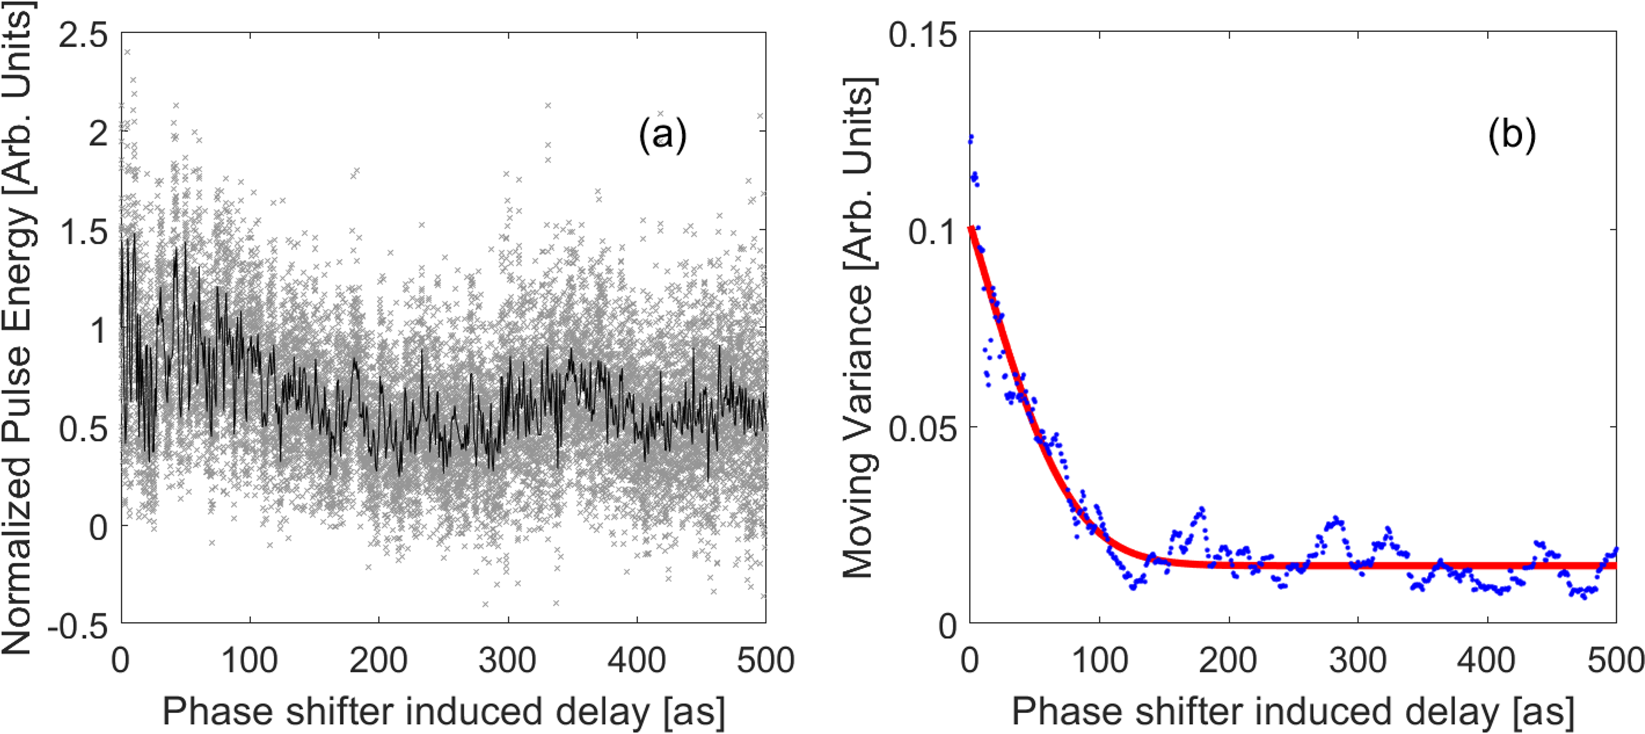
\includegraphics[width=0.8\textwidth]{Figuras/ch1_coher.png}
  \caption{Resultados experimentales del tiempo de coherencia medidos en el \acrshort{lcls}\autocite{zhouAttosecondCoherenceTime2020}. \textbf{a}, Energía de los pulsos frente al retraso temporal. \textbf{b}, Cambios en la varianza respecto al retraso temporal.}
  \label{fig:ch1_coher}
\end{figure}

El concepto de coherencia de primer orden hace referencia a que la medición realizada contempla la correlación entre amplitudes de ondas --el campo eléctrico---, mientras que la coherencia de orden $n$ expresa la correlación entre los productos de orden $n$ del campo eléctrico. Por ejemplo, a segundo orden ---el cuadrado del campo eléctrico---, la medición encierra la información sobre la intensidad del campo, de manera que la \emph{función correlación de orden} $n$ sería $\Gamma^{(n)}(\symbf{r}_1,t_1,\ldots,\symbf{r}_n,t_n) = \langle E(\symbf{r}_1,t_1)E^{*}(\symbf{r}_1,t_1)\ldots E(\symbf{r}_n,t_n)E^{*}(\symbf{r}_n,t_n)\rangle$.

\paragraph{Direccionalidad}\label{par:1.1.2.3}
La emisión de un láser puede llegar a consistir en frentes de onda planos prácticamente ideales. La difracción es el único fenómeno ondulatorio que impone un umbral inferior en la divergencia del haz láser. El orden de magnitud del ángulo sólido $\Delta\Omega$ y el ángulo de divergencia $\Delta\theta$ dependen fundamentalmente de la longitud de onda $\lambda$ y el área de apertura $A$ de la emisión\autocite{milonniLasers1988} a través de la relación
\begin{equation}\label{eq:1.3}
    \Delta\Omega \approx \frac{\lambda^{2}}{A} \approx (\Delta\theta)^{2}.
\end{equation}
Para longitudes de onda en el rango óptico, por ejemplo, $\lambda = \qty{500}{nm}$, y con una superficie de salida de la cavidad habitual de $A = \qty{5}{mm^2}$, la relación \eqref{eq:1.3} proporciona una divergencia de $\Delta\theta = \sqrt{\qty{250000e-18}{m^2}/(\qty{25e-6}{m^2})} = \qty{0,1}{mrad}$. Con ángulos de divergencia similares a este ejemplo, que son habituales en láseres, como muestra la Tabla \ref{tab:1.1}, el llamado \emph{rango de Rayleigh} permite caracterizar la distancia recorrida $z$. En este rango, el ancho $w_0$ del haz láser se incrementa en un factor $\sqrt{2}$ en el plano transversal, siendo aproximadamente en este caso
\begin{equation}\label{eq:1.4}
    z\approx\frac{A}{\lambda} = \frac{\qty{5e-6}{m^2}}{\qty{500e-9}{m}} = \qty{10}{m}.
\end{equation}

Para áreas de apertura mayores, por ejemplo $A = \qty{5}{cm^2}$, la distancia aumenta hasta alcanzar $z = \qty{1}{km}$. Empleando menores longitudes de onda el rango sería incluso mayor, dando una idea de las largas distancias capaces de recorrer muchos láseres sin pérdida de direccionalidad.

\begin{table}[ht!]
  \centering
  \caption{Ángulos de divergencia típicos en láseres\autocite{milonniLasers1988}.}
  \begin{tabular}{ccc}
    \toprule
     Láser           & $\Delta\theta$ (\unit{mrad}) & $\Delta\Omega$ (\unit{sr}) \\
    \midrule
    \ce{He-Ne}      & $0,2-1$                                & $(0,1-3)\times 10^{-6}$ \\
    \midrule
    \ce{CO2}        & $1-10$                                  & $(3-300)\times 10^{-6}$ \\
    \midrule
    Rubí            & $1-10$                                  & $(3-300)\times 10^{-6}$ \\
    \midrule
    \ce{Nd{:}YAG}     & $1-20$                                & $(3-1300)\times 10^{-6}$ \\
    \midrule
    \ce{Nd{:}cristal} & $0,5-10$                              & $(1-300)\times 10^{-6}$ \\
    \bottomrule
  \end{tabular}
  \label{tab:1.1}
\end{table}

\paragraph{Luminosidad}\label{par:1.1.2.4}
Un haz de luz procedente de una fuente puede caracterizarse por la divergencia del haz $\Delta\Omega$, el tamaño de la fuente ---normalmente una superficie de área $A$---, el ancho de banda $\Delta\nu$ y la densidad de potencia de la emisión $P(\nu)$, es decir, la potencia por unidad de frecuencia del ancho de banda\autocite{milonniLasers1988}. A partir de estos parámetros, es interesante definir la \emph{luminosidad espectral} $\beta_{\nu}$ de la fuente como 
\begin{equation}\label{eq:1.5}
    \beta_{\nu} = \frac{P(\nu)}{A\Delta\Omega\Delta\nu} = \frac{I(\nu)}{\Delta\Omega},
\end{equation}
con $I(\nu)$ la intensidad espectral del haz de luz, de manera que también puede definirse $\beta_{\nu}$ como la intensidad espectral por unidad de ángulo sólido.

Para una fuente de radiación ordinaria, esta luminosidad puede estimarse directamente suponiendo la expresión de la densidad espectral de energía $\rho(\nu)$ de un cuerpo negro. Empleando la ecuación \eqref{eq:1.5} y la hipótesis del cuerpo negro ($\Delta\Omega=4 \pi$), resulta
\begin{equation}\label{eq:1.6}
    \beta_{\nu} = \frac{c \rho(\nu)}{4 \pi} = \frac{2 \nu^{2}}{c^{2}}\frac{h \nu}{\eu^{h \nu/kT}-1}.
\end{equation}
La temperatura de la superficie del sol es aproximadamente $T = \qty{5800}{K} \approx 20 \times \qty{300}{K}$. La mayoría de la emisión del sol está en la franja amarilla de la banda visible, de forma que $h\nu \approx \qty{2,5}{eV}$ ($\nu \approx \qty{5e14}{Hz}$ para un fotón en el amarillo-verde). Para $T = \qty{300}{K}$ se tiene $kT \approx \qty{0,025}{eV}$, por tanto, $h \nu/kT \approx 5$, obteniéndose $\eu^{h \nu/kT}-1 \approx 150$ y, finalmente,
\begin{equation}\label{eq:1.7}
    \beta_{\nu} \approx \qty{1,5e-12}{W/cm^{2}\,sr\,Hz}.
\end{equation}
Dependiendo del tipo de láser pueden hacerse varias estimaciones. Escogiendo un láser \ce{He-Ne} de baja potencia, valores típicos\autocite{milonniLasers1988} son potencias de \qty{1}{mW} con anchos de banda en torno a \qty{e4}{Hz}. A partir de la ecuación \eqref{eq:1.3}, puede calcularse la longitud de onda como $\lambda^{2} \approx A\Delta\Omega$, que para la luz del láser \ce{He-Ne} es $\lambda^{2} \approx (\qty{6238e-8}{cm})^{2} \approx \qty{3,89e-9}{cm^{2}}$. Combinando estos datos, resulta 
\begin{equation}\label{eq:1.8}
    \beta_{\nu} \approx \qty{26}{W/cm^{2}\,sr\,Hz}.
\end{equation}
Con láseres de mayor potencia, como el láser de \ce{Nd{:}cristal}, que puede alcanzar potencias de \qty{e4}{MW}, su luminosidad es $\beta_{\nu} \approx \qty{2e8}{W/cm^{2}\,sr\,Hz}$, y para las potencias de teravatios (\qty{1}{TW} = \qty{e6}{MW}) alcanzadas en algunos láseres, la luminosidad es varios órdenes de magnitud más elevada.

De esta manera, el concepto de luminosidad deja patente la existencia de grandes diferencias entre las fuentes de radiación convencionales y los láseres. Incluso atenuando la luminosidad del láser \ce{He-Ne} hasta alcanzar el valor de la radiación solar y, por otro lado, colimando y filtrando la radiación solar hasta alcanzar la direccionalidad y el ancho de banda del láser \ce{He-Ne}, podrían distinguirse ambas fuentes, contando los fotones emitidos para detectar pequeñas fluctuaciones estadísticas debidas a la naturaleza cuántica de la luz. 

\paragraph{Duración}\label{par:1.1.2.5}
Esta propiedad está relacionada con la monocromaticidad explicada en la sección \S\ref{par:1.1.2.1}. La duración de un pulso láser determina su densidad de energía en el tiempo, que puede considerarse inversamente proporcional a la densidad de energía en la longitud de onda, esto es, su monocromaticidad\autocite{sveltoPrinciplesLasers2010}. Teóricamente, cualquier tipo de láser puede ser tan monocromático como sea necesario, pero los pulsos de muy corta duración solo pueden generarse, por ejemplo, en láseres de estado sólido o láseres de líquido, donde el ancho de banda es suficientemente amplio.

Empleando una técnica ---habitual en algunos láseres con pulsos ultracortos--- conocida como \emph{mode locking} que, sin entrar en profundidad en este método, consiste en establecer una relación fija entre las fases de los modos longitudinales de oscilación que se forman en la cavidad resonante, es posible producir pulsos de luz con una duración aproximadamente igual al inverso del ancho de banda para la transición $2 \rightarrow 1$. Por ejemplo, en láseres de gas, cuyo ancho de banda es relativamente pequeño, la duración del pulso puede ser $\sim\qty{0,1}{ns}-\qty{1}{ns}$. Esta duración no es especialmente corta teniendo en cuenta que algunas lámparas flash pueden emitir pulsos de luz inferiores a \qty{1}{ns}. Por otra parte, el ancho de banda de algunos láseres de estados sólido o láseres de líquido puede ser $10^3-10^5$ veces mayor que en los láseres de gas, generando pulsos extremadamente cortos (hasta $\sim\qty{10}{fs}$).

La longitud de onda y la duración del pulso tienen especial importancia en muchas aplicaciones tecnológicas y en investigación, por ejemplo, en la reconstrucción de imágenes tridimensionales de moléculas\autocite{vonardenneStructureDeterminationSingle2018}, bacterias o virus\autocite{ekebergThreeDimensionalReconstructionGiant2015}, donde la resolución necesaria para visualizar escalas extremadamente pequeñas requiere longitudes de onda de nanómetros ($\sim\qty{e-9}{m}$) o ángstroms ($\sim\qty{e-10}{m}$) y pulsos con duraciones de femtosegundos ($\sim\qty{e-15}{s}$) o incluso attosegundos ($\sim\qty{e-18}{s}$). Estas técnicas están basadas en formar cientos de patrones de difracción entre el pulso láser y el blanco objeto de estudio, para después emplear métodos de análisis de Fourier que permiten obtener imágenes tridimensionales a partir de los patrones de difracción bidimensionales, como muestra la Figura \ref{fig:ch1_pulso}.

\begin{figure}[ht!]
  \centering
  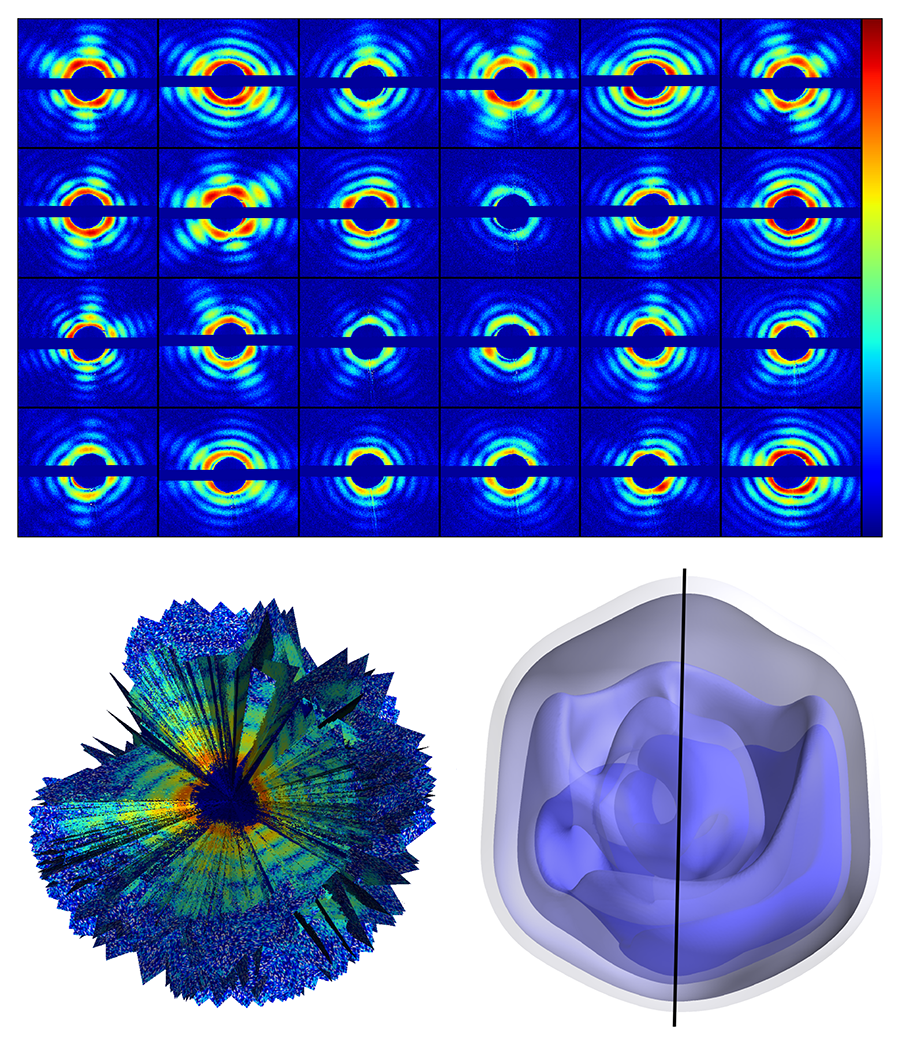
\includegraphics[width=0.5\textwidth]{Figuras/ch1_pulso.png}
  \caption{Patrones de difracción y densidad de electrones obtenida de un \enquote{Mimivirus}\autocite{ekebergThreeDimensionalReconstructionGiant2015}. La resolución conseguida es de \qty{125}{nm}. El tamaño de la envoltura del virus es aproximadamente de \qty{450}{nm}.}
  \label{fig:ch1_pulso}
\end{figure}

El aspecto clave del ancho de pulso en estas aplicaciones está en conseguir la difracción antes destruir completamente la muestra\autocite{neutzePotentialBiomolecularImaging2000}, motivando la necesidad de pulsos extremadamente cortos o ultracortos ($\le\unit{fs}$) para visualizar imágenes. Por otro lado, el papel de la longitud de onda es conseguir la resolución necesaria para observar menores tamaños, ya que longitudes de onda mayores que el tamaño característico del objeto que quiere estudiarse no permiten exhiben el fenómeno de difracción necesario. En la actualidad ---se explicará más detalladamente en la sección \S\ref{sec:1.3}---, las únicas fuentes de radiación que reúnen estos requisitos son los láseres de rayos X blandos o \emph{\acrfull{sxrl}}.

\section{Plasma}\label{sec:1.2}

\subsection{Propiedades físicas}\label{sec:1.2.1}

\subsection{Ondas electromagnéticas en plasmas}\label{sec:1.2.2}

\subsection{Interacción láser-plasma}\label{sec:1.2.3}

\section{Fuentes de radiación X coherente}\label{sec:1.3}

\subsection{Radiación sincrotrón}\label{sec:1.3.1}

\subsection{Láseres de electrones libres}\label{sec:1.3.2}

\subsection{Armónicos de alto orden}\label{sec:1.3.3}

\subsection{Radiación betatrón}\label{sec:1.3.4}

\section{Láseres de rayos X basados en plasmas}\label{sec:1.4}

\section{Estado del arte}\label{sec:1.5}
